\documentclass[11pt,a4paper,titlepage, oneside]{article}

\usepackage[T1]{fontenc}
\usepackage[utf8x]{inputenc}
\usepackage{graphicx} 	% images
\usepackage{wrapfig}
\usepackage{listings}
\usepackage{url}
\usepackage{times}
\usepackage[T1]{fontenc}      % caracteres francais
\usepackage{xcolor}		%couleurs
\usepackage[frenchb]{babel}  % langue
\usepackage{geometry}         % marges
\usepackage{verbatim}  
\usepackage{moreverb}       % texte preformate
\usepackage{array}
%\usepackage[linktocpage,colorlinks=true]{hyperref}
\usepackage[final]{pdfpages}

%Définition de l'apparence des listings
\lstset{
	frame=single,
	breaklines=true,
	basicstyle=\small,
	mathescape=false
}


%Le titre de projet
\title{Projet 4A STI : Supervision et audit de la sécurité système dans un réseau}

%Votre nom
\author{Aymeric Berquin \and Fayçal-Anoar Cherkaoui}

%Par défaut, Latex utilise la date du jour
%Pour supprimer la date ou la changer:
\date{1 Janvier 2015}
\geometry{top=3cm, bottom=3.5cm, left=3cm , right=2.5cm}


\begin{document}
%Créer la page de titre
\begin{titlepage}
 \thispagestyle{empty}
\begin{figure}[h]
  \centering
  
\includegraphics[width=0.8\textwidth,natwidth=610,natheight=642]{images/logo.png}
\end{figure}
\vspace{0,5cm}
\begin{center} 
\Huge{\textbf{{\color{red}}}Projet 2A STI : Supervision et audit de la sécurité système dans un réseau}
\\
\vspace{1.5 cm}

\vspace{1cm}
\large{Diplôme d'Ingénieur, 4e année}
\\
\vspace{1cm}
\large{Aymeric Berquin \\ \& \\ Fayçal-Anoar Cherkaoui}
\vspace{1 cm}
\paragraph{}
	\Large{Date de rendu de rapport : 12/02/2015}
	\\
	
\vspace{1.5 cm}
\end{center} 
\end{titlepage} 
\normalsize
\newpage
\section*{\textbf{Remerciement}}
\thispagestyle{empty}
	\paragraph{}
	Nous remercions Monsieur Briffaut pour le temps et les ressources qu'il nous a consacré. Nous le remercions aussi pour toutes les connaissances qu'il nous a apportés.

\newpage
\section*{{\color{red}Introduction}}
	\paragraph{}
		Dans le cadre de notre formation d'ingénieurs en Sécurité et Technologies Informatiques, un projet d'application sécurité nous est soumis. Dans notre cas il s'agit de concevoir une application client/serveur permettant la supervision et l'audit de la sécurité dans un réseau. Il s'agit de nous mettre en situation de travail en binôme  sur un projet donné et sur un moyen terme. 
		
		
\newpage
\thispagestyle{empty}
\tableofcontents
\listoffigures  % table des figures

\newpage
\pagenumbering{arabic} \setcounter{page}{1}
\section{{\color{red}Installation des machines virtuelles}}
\subsection{{\color{blue}{Installation du serveur Debian}}}
	\paragraph{}
		Installation d'un debian classique sans interface graphique, qui jouera le rôle du maitre.
		
		On récupère l'iso sepuis le site officiel: http://www.ubuntu.com/download/desktop.

		On configure les caractéristiques suivantes:
		\begin{itemize}
                        \item{1GB en RAM}
                        \item{1 processeur}
                        \item{20GB en dique dur}
                \end{itemize}
 		\paragraph{}
		On choisi une installation sans interface graphique.
		 \begin{figure}[h]
                        \centering
                        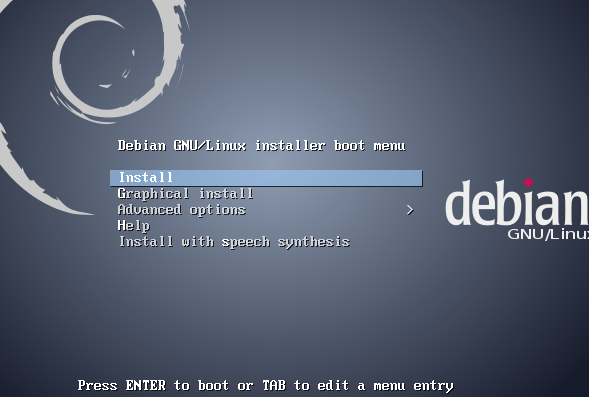
\includegraphics[width=0.8\textwidth,natwidth=610,natheight=642]{images/debian1.png}
                        \caption{choix de linstallation}
                \end{figure}
		

	\newpage		
		\begin{figure}[h]
                        \centering
                        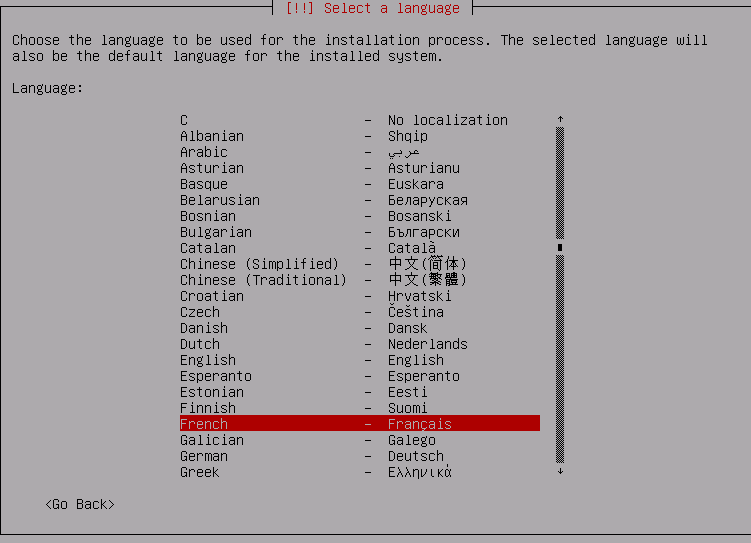
\includegraphics[width=0.8\textwidth,natwidth=610,natheight=642]{images/debian2.png}
                        \caption{choix de la langue}
                \end{figure}
	\newpage
		\begin{figure}[h]
                        \centering
                        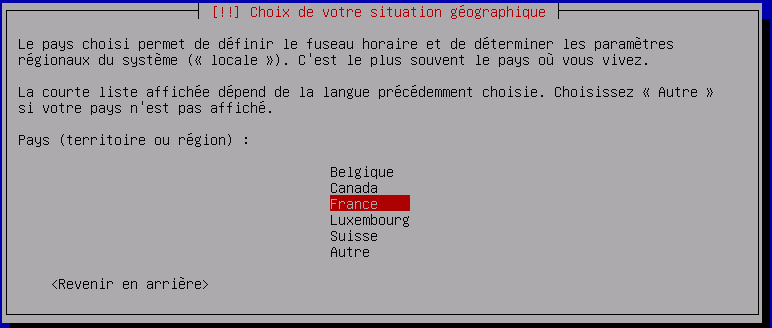
\includegraphics[width=0.8\textwidth,natwidth=610,natheight=642]{images/debian3.png}
                        \caption{choix de la localisation géographique}
                \end{figure}


	\newpage
                \begin{figure}[h]
                        \centering
                        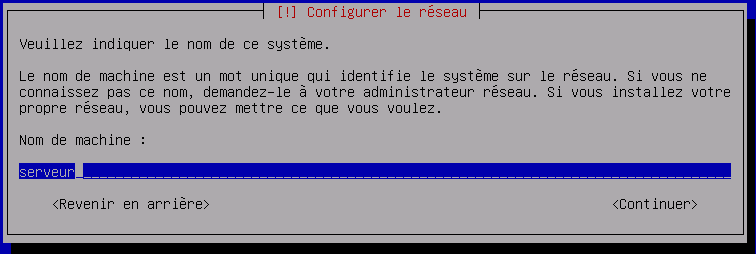
\includegraphics[width=0.8\textwidth,natwidth=610,natheight=642]{images/debian4.png}
                        \caption{Nom de l'hôte: hostname}
                \end{figure}

	 \newpage
                \begin{figure}[h]
                        \centering
                        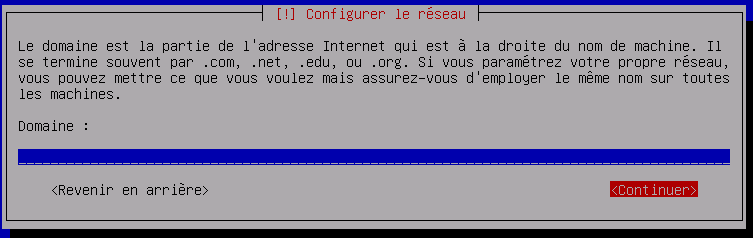
\includegraphics[width=0.8\textwidth,natwidth=610,natheight=642]{images/debian5.png}
                        \caption{Nom du domaine de la machine}
                \end{figure}

	 \newpage
                \begin{figure}[h]
                        \centering
                        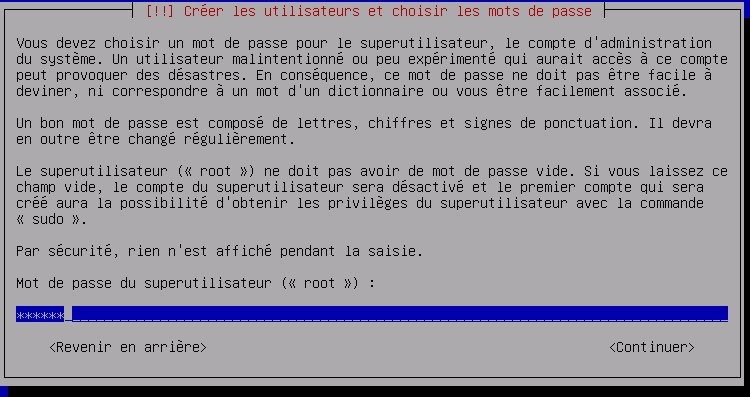
\includegraphics[width=0.8\textwidth,natwidth=610,natheight=642]{images/debian6.png}
                        \caption{Définition du mot de passe du compte root}
                \end{figure}


	 \newpage
                \begin{figure}[h]
                        \centering
                        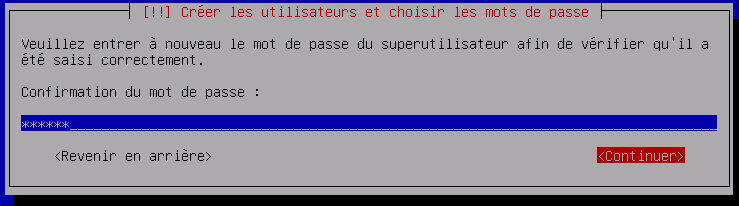
\includegraphics[width=0.8\textwidth,natwidth=610,natheight=642]{images/debian7.png}
                        \caption{Confirmation du mot de passe}
                \end{figure}

	 \newpage
                \begin{figure}[h]
                        \centering
                        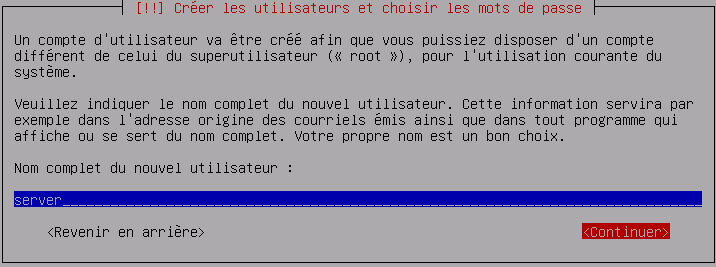
\includegraphics[width=0.8\textwidth,natwidth=610,natheight=642]{images/debian8.png}
                        \caption{Création d'un compte utilisateur}
                \end{figure}

	 \newpage
                \begin{figure}[h]
                        \centering
                        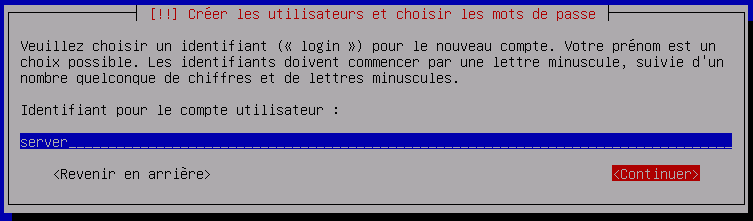
\includegraphics[width=0.8\textwidth,natwidth=610,natheight=642]{images/debian9.png}
                        \caption{Choix du login du compte utilistauer précédemment créé}
                \end{figure}

	 \newpage
                \begin{figure}[h]
                        \centering
                        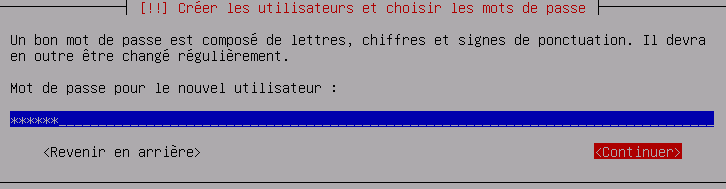
\includegraphics[width=0.8\textwidth,natwidth=610,natheight=642]{images/debian10.png}
                        \caption{Définition du mot de passe pour le compte utilisateur}
                \end{figure}

	
	\newpage
                \begin{figure}[h]
                        \centering
                        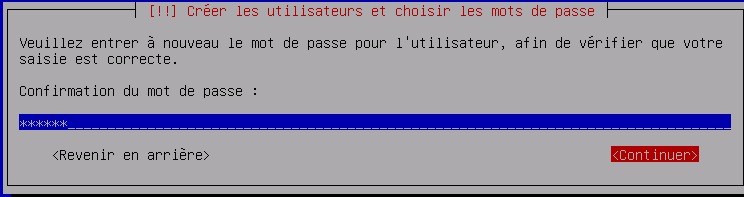
\includegraphics[width=0.8\textwidth,natwidth=610,natheight=642]{images/debian11.png}
                        \caption{confirmation du mot de passe pour le compte utilisateur}
                \end{figure}

	 \newpage
                \begin{figure}[h]
                        \centering
                        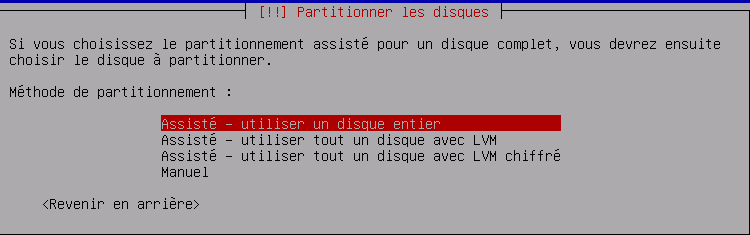
\includegraphics[width=0.8\textwidth,natwidth=610,natheight=642]{images/debian12.png}
                        \caption{Partitionnement du disque}
                \end{figure}

	 \newpage
                \begin{figure}[h]
                        \centering
                        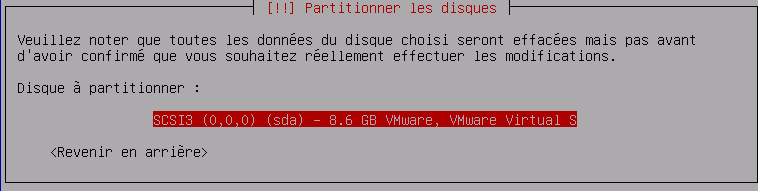
\includegraphics[width=0.8\textwidth,natwidth=610,natheight=642]{images/debian13.png}
                        \caption{Partitionnement du disque}
                \end{figure}


		 \newpage
                \begin{figure}[h]
                        \centering
                        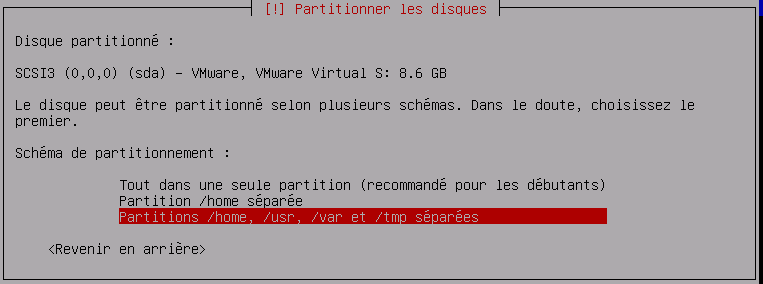
\includegraphics[width=0.8\textwidth,natwidth=610,natheight=642]{images/debian14.png}
                        \caption{Partitionnement du disque}
                \end{figure}

	\newpage
                \begin{figure}[h]
                        \centering
                        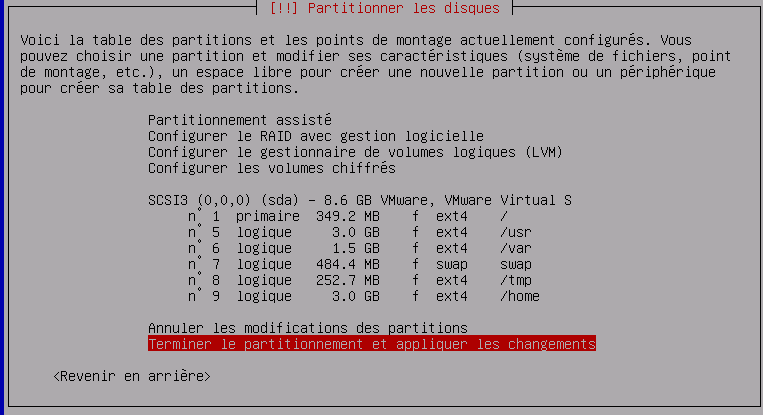
\includegraphics[width=0.8\textwidth,natwidth=610,natheight=642]{images/debian15.png}
                        \caption{Partitionnement du disque}
                \end{figure}

	\newpage
                \begin{figure}[h]
                        \centering
                        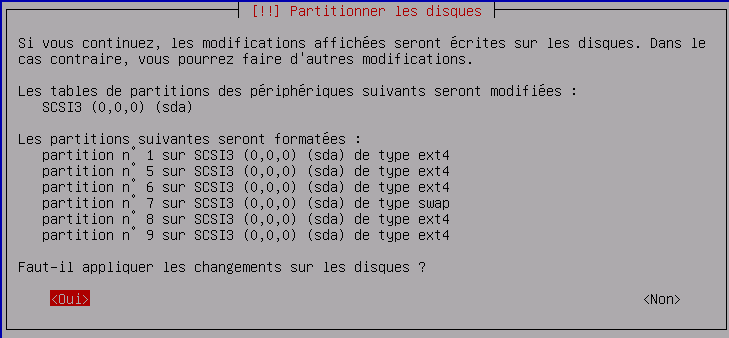
\includegraphics[width=0.8\textwidth,natwidth=610,natheight=642]{images/debian16.png}
                        \caption{Partitionnement du disque}
                \end{figure}

	\newpage
                \begin{figure}[h]
                        \centering
                        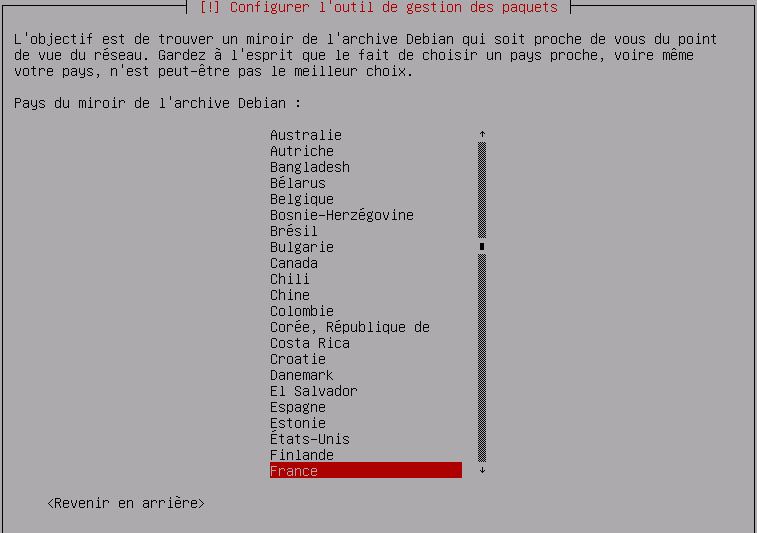
\includegraphics[width=0.8\textwidth,natwidth=610,natheight=642]{images/debian17.png}
                        \caption{Configuration de l'outil de gestion du paquet}
                \end{figure}

	\newpage
                \begin{figure}[h]
                        \centering
                        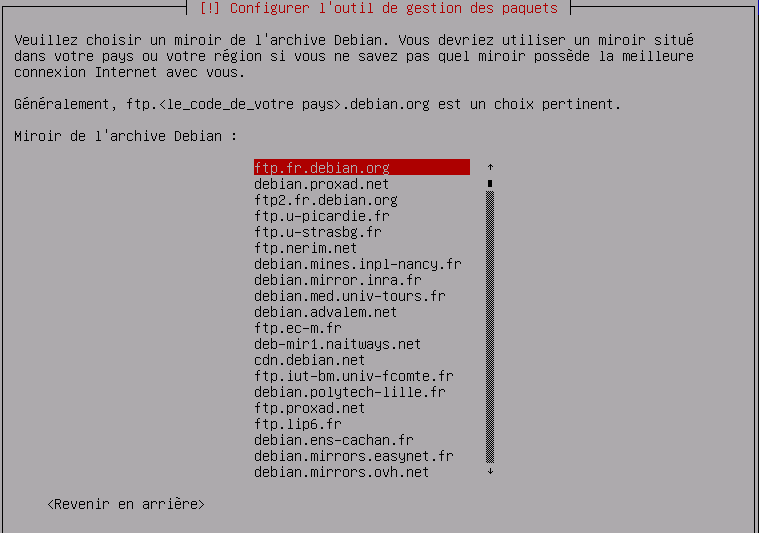
\includegraphics[width=0.8\textwidth,natwidth=610,natheight=642]{images/debian18.png}
                        \caption{Configuration de l'outil de gestion du paquet}
                \end{figure}

	\newpage
                \begin{figure}[h]
                        \centering
                        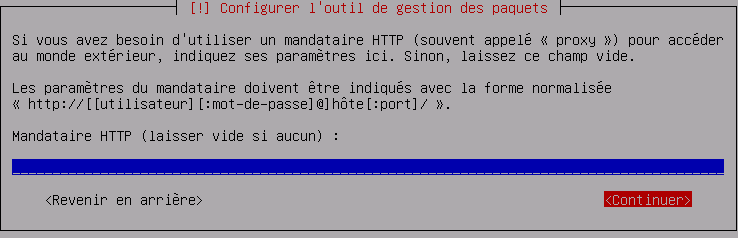
\includegraphics[width=0.8\textwidth,natwidth=610,natheight=642]{images/debian19.png}
                        \caption{configuration de l'outil de gestion du paquet}
                \end{figure}

	\newpage
                \begin{figure}[h]
                        \centering
                        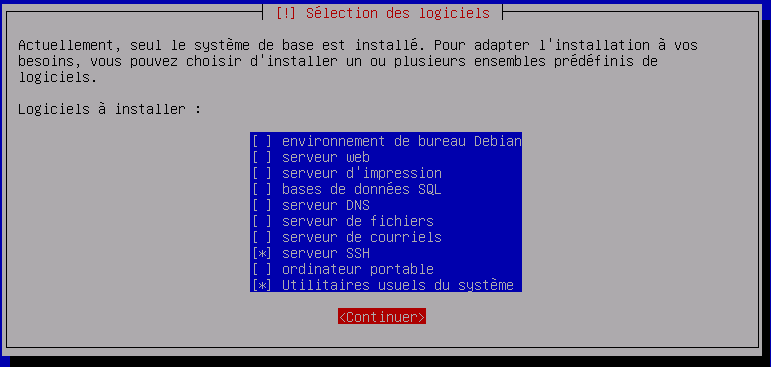
\includegraphics[width=0.8\textwidth,natwidth=610,natheight=642]{images/debian20.png}
                        \caption{Sélection des logiciels}
                \end{figure}

	\newpage
                \begin{figure}[h]
                        \centering
                        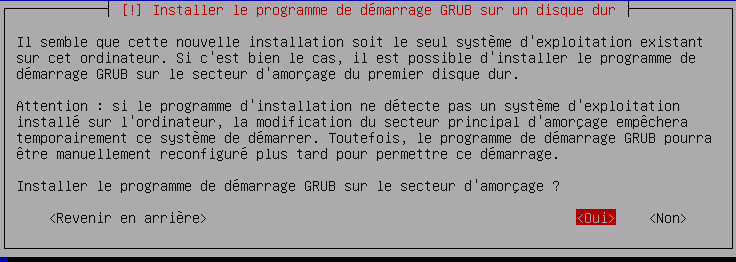
\includegraphics[width=0.8\textwidth,natwidth=610,natheight=642]{images/debian21.png}
                        \caption{Installation du programme de démarrage GRUB}
                \end{figure}

	\newpage
                \begin{figure}[h]
                        \centering
                        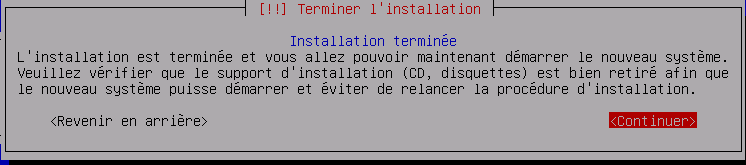
\includegraphics[width=0.8\textwidth,natwidth=610,natheight=642]{images/debian22.png}
                        \caption{Fin de l'installation}
                \end{figure}
\subsection{{\color{blue}{Installation du client ubuntu}}}
\paragraph{}
	        On aura besoin d'installer deux machines virtuelles avec la dernière distribution Ubuntu stable. Elles auront pour nom client1 et client2.

		Nous avons choisi d'utiliser un Xubuntu 14.04. A récuperer sur le site officiel: http://www.ubuntu.com/download/desktop
		
		Nom complet : user
			
		Nom d'utilisateur : user
		
		Mot de passe : resu
		
		Hostname : client1
		
		\begin{figure}[h]
  			\centering
  			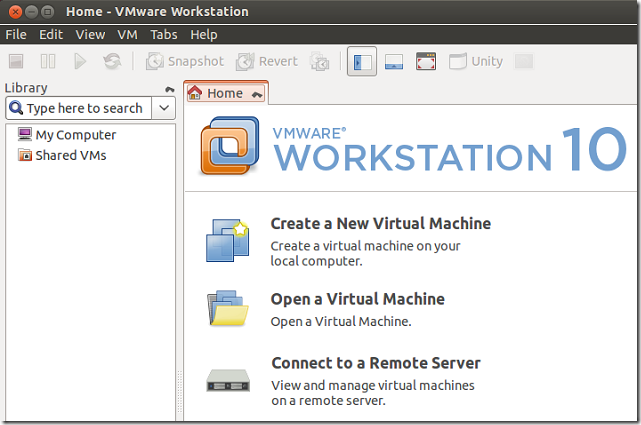
\includegraphics[width=0.8\textwidth,natwidth=610,natheight=642]{images/vmwareworkstationubuntu.png}
			\caption{interface de la machine virtuelle VMware}
		\end{figure}
		Elle aura pour configuration:
		\begin{itemize}
                        \item{1GB en RAM}
                        \item{1 processeur}
                        \item{20GB en dique dur}
                \end{itemize}
		On éditera la nouvelle machine virtuelle VMware dans laquelle en spécifiant le chemin de l'iso téléchargé.
		
		On démarre la machine virtuelle.
	\newpage
		\begin{figure}[h]
                        \centering
                        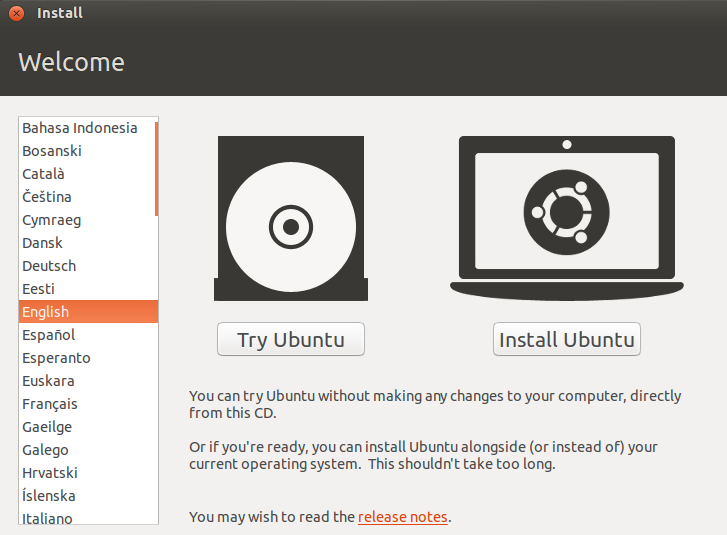
\includegraphics[width=0.8\textwidth,natwidth=610,natheight=642]{images/demarrerISO.png}
                        \caption{Choix de la langue d'installation}
                \end{figure}
		Une nouvelle fenêtre s'affiche, on clique sur suivant.
		 \begin{figure}[h]
                        \centering
                        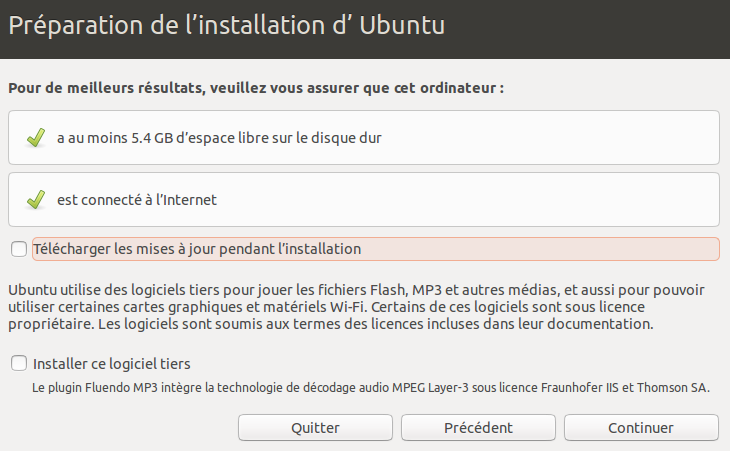
\includegraphics[width=0.8\textwidth,natwidth=610,natheight=642]{images/demarrerISO2.png}
                        \caption{Prérequis pour l'installation}
                \end{figure}
	\newpage
		On procédera à une installation par défaut.
		 \begin{figure}[h]
                        \centering
                        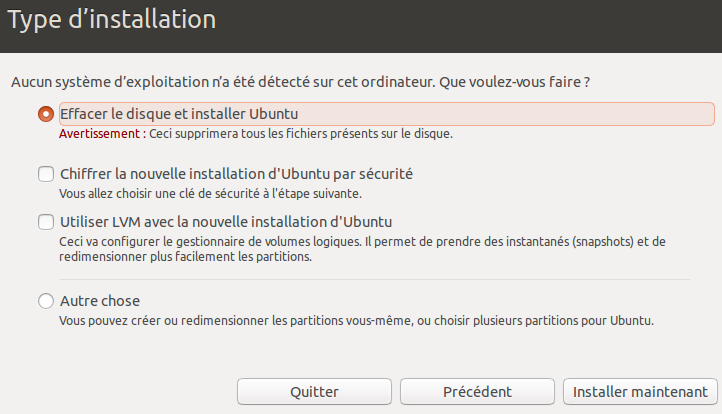
\includegraphics[width=0.8\textwidth,natwidth=610,natheight=642]{images/demarrerISO3.png}
                        \caption{Type d'installation}
                \end{figure}
		
	\newpage
		Une nouvelle fenêtre pour le choix du fuseau horaire. On choisie Paris.
		 \begin{figure}[h]
                        \centering
                        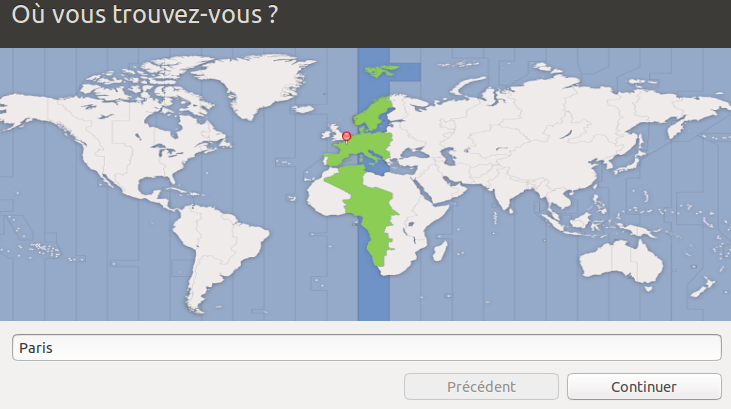
\includegraphics[width=0.8\textwidth,natwidth=610,natheight=642]{images/demarrerISO4.png}
                        \caption{Choix du fuseau horaire.}
                \end{figure}
	\newpage
		La nouvelle fenêtre qui s'affiche est pour le choix de la disposition du clavier.

		 \begin{figure}[h]
                        \centering
                        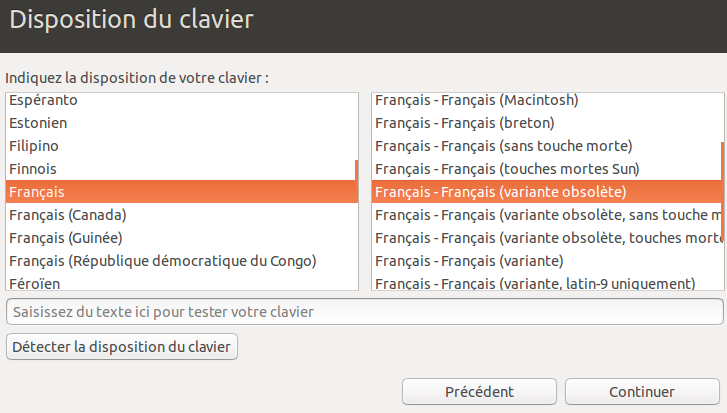
\includegraphics[width=0.8\textwidth,natwidth=610,natheight=642]{images/demarrerISO5.png}
                        \caption{Disposition du clavier.}
                \end{figure}

		\newpage

		On procède dans cette étape à la création du client1.	
		\begin{figure}[h]
                        \centering
                        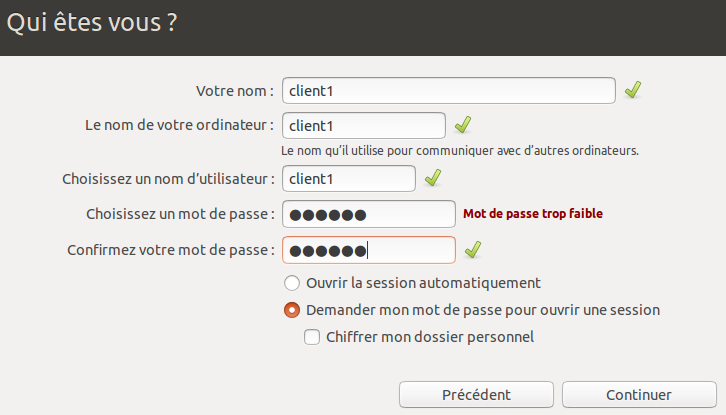
\includegraphics[width=0.8\textwidth,natwidth=610,natheight=642]{images/demarrerISO6.png}
                        \caption{Création du client1.}
                \end{figure}

		\newpage
		On redémarre la machine.

	\begin{figure}[h]
                        \centering
                        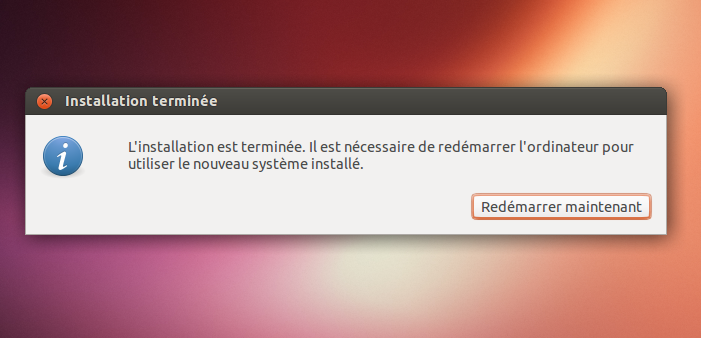
\includegraphics[width=0.8\textwidth,natwidth=610,natheight=642]{images/demarrerISO7.png}
                        \caption{Redémarrage de la machine.}
                \end{figure}
	
		On est arrivé à la fin de l'installation de la machine client1, pour le deuxième client il nous suffit de faire un clone du premier client. UN clic droit sur la machine client1 puis manage puis clone.

	On démarre la machine clonnée puis dans /etc/hostname on modifie le nom en la nommant client2.
		\colorbox{gray}{vim /etc/hostname}

	
\newpage
\section{{\color{red} Git}}
	\paragraph{}
		Nous avons décidé d'utiliser un serveur git pour gérer les sources.
		
		Git est un logiciel de gestion de versions décentralisé. C'est-à-dire que le développement ne se fait pas sur un serveur centralisé, mais chaque personne peut développer sur son propre dépôt. Git facilite ensuite la fusion (merge) des différents dépôts.

		Pour pouvoir utiliser Git, il suffit d'installer le paquet git:
	
		\colorbox{gray} {apt-get install git}

	\subsection{{\color{blue} Gérer les dépots}}
		\paragraph{}
			Pour pouvoir utiliser le Git il va falloir tout d'abord créer un dépot.
			
			\colorbox{gray}{mkdir proscan

				cd proscan
	
				git init}
	
	\subsection{{\color{blue} Etat du dépot}}	
		\paragraph{}
			\colorbox{gray}{git diff git diff <commit1> <commit2>}

			Le git offre la possiblité de trouver les changements éffectués. SI vous avez des changements pas encore commités, la commande git diff affichera les modifications éffectuées depuis le dernier commit.

			\colorbox{gray}{git status} Permet de savoir tout ce qui n'a pas encore été validé.
	
			\colorbox{gray}{git log} Liste les commits éffectués dans le dépot. Et ainsi voir les modifications faites dans quelle date et par qui.

	\subsection{{\color{blue} Gestion des fichiers}}

		\paragraph{}
			Pour ajouter au git un dossier ou un fichier on utilise la commande:

			\colorbox{gray}{git add <nom-du fichier-ou-du-dossier>}

			Pour ajouter tout le contenu d'un fichier ou d'un dossier:

			\colorbox{gray}{git add *}

			Pour supprimer le fichier de l'ordinateur, ainsi que du dépot git:		
			
			\colorbox{gray}{git rm <nom-fichier>}

			Pour dépolacer le fichier de l'ordinateur, ainsi que du dépot Git:
			
			\colorbox{gray}{git mv <nom-fichier> <nouvel-emplacement>}

	\subsection{{\color{blue} Gestion des commits}}

		\paragraph{}
			Met à jour votre dépôt local (à faire avant de commencer à modifier des fichiers pour être sûr de travailler sur leurs dernières versions et avant tout commit pour éviter les éventuels conflits avec des modifications effectuées par d'autres utilisateurs entre temps). 

			\colorbox{gray}{git pull}

			Créer un commit contenant fichier1 et fichier2. Ces fichiers auront dû être au préal able ajoutés au dépôt avec la commande git add. Il s'agit de la validation d'une transaction. 

			Pour envoyer un commit dans la branche principale du dépot (master):
			
			\colorbox{gray}{git push origin master}	

\newpage
\section{{\color{red} Base De Données}}
	\subsection{{\color{blue}Client}}
		\paragraph{Table Client}
			La table client est constituée de :
			\begin{itemize}
				\item id : identifiant auto-indexé, clé primaire
				\item ip : adresse ip du client
				\item hmac : hmac du client (unique)
				\item hostname : Nom d'hôte du client
				\item pid : pid du processus chargé de communiquer avec ce client
			\end{itemize}
	\subsection{{\color{blue} Script}}
		\paragraph{Table Script}
			La table script est constituée de :
			\begin{itemize}
				\item id : identifiant auto-indexé, clé primaire
				\item nom : Nom du script
				\item description : Description rapide du script
				\item code : code du script
			\end{itemize}
	\subsection{{\color{blue}Result}}
		\paragraph{Table Result}
			La table result qui enregistre les résultats des scripts est constituée de :
			\begin{itemize}
				\item id : identifiant auto-indexé, clé primaire
				\item idclient : Identifiant du client
				\item idscrip : Identifiant du script
				\item result : résultat du script
			\end{itemize}
		
		
\newpage
\section{{\color{red} Client/Serveur}}

\newpage
\section{{\color{red} Interface WEB}}

\newpage
\section{{\color{red} Script }}
	\paragraph{Permissions}
		Bien que la majorité de nos scripts puissent s'exécuter avec les permissions d'un utilisateur, certain d'entre eux nécessites les droits d'administrateur.\\
	\subsection{{\color{blue}En Tant qu'utilisateur}}
		\begin{tabular}{|l|p{12cm}|}
			\hline
				\textbf{N°}&\textbf{Résultats}\\
			\hline
				1 & Hostname, Interfaces réseaux, nom de la distribution, version de la distribution, version du noyau, table de routage.\\
			\hline
				2 & Espace des partitions montées.\\
			\hline
				3 & Affiche les connections internet actives.\\
			\hline
				4 & Processus actif.\\
			\hline
				5 & Variables d'environnement.\\
			\hline
				6 & Informations CPU, Interruptions, Mémoire utilisée, Fichier\(s\) Swap\(s\), version du noyau,systèmes de fichiers montés, périphériques CPU, périphériques usb.\\
			\hline
				7 & Affiche les processus en cours dans une arborescence qui commence à la racine.\\
			\hline
				8 & Récupération de tous les fichiers d'extension ".log".\\
			\hline
				9 & Table de routage.\\
			\hline
				10 & interfaces réseaux.\\
			\hline
				11 & User loggé, heure du dernier démarrage, affiche les processus morts, runlevel courant.\\
			\hline
				13 & Liste des utilisateurs.\\
			\hline
				14 & Affiche l'état de la mémoire de la partition courante.\\
			\hline
				17 & Vérification de l'intégrité de /bin, /usr/bin, /sbin, /usr/sbin.\\
			\hline
		\end{tabular}
			
	\subsection{{\color{blue}En Tant qu'administrateur}}
		\begin{tabular}{|l|p{12cm}|}
			\hline
			\textbf{N°}&\textbf{Résultats}\\
				15 & Affichage de la dernière connexion local.\\
			\hline
				16 & Affiche les règles iptables pour filter, nat et mangle .\\
			\hline
		\end{tabular}
		
\newpage
\section{{\color{red}Conclusion}}
	

%\newpage
%\section{{\color{red}Évolution temporelle}}
%\begin{tabular}{|l|p{12cm}|}
%	\hline
%		
%		\textbf{DATE}& \textbf{OBJET} \\
%		
%	\hline
%		10/09/14 & Présentation du projet et formation du binôme\\
%	\hline
%		17/09/14 & Début rapport. Étude du sujet. Installation VM Client\\
%	\hline
%		24/09/14 & Début client/server\\
%	\hline
%		01/10/14 & Rédaction des Makefiles de base\\
%	\hline
%		08/10/14 & Correction erreur client/serveur\\
%	\hline
%		07/11/14 & Fonction client exécution de script\\
%	\hline
%		10/11/14 & Premier scan. Création fonction de log client\\
%	\hline
%		19/11/14 & Autres script\\
%	\hline
%		03/12/14 & script mémoire + pattern script\\
%	\hline
%		08/12/14 & Scripts, ajout de la description des scripts au rapport\\
%	\hline
%		
%		
%
%\end{tabular}
		



\newpage
\section{{\color{red}Bibliographie}}
%\thispagestyle{empty}		
	\subsection*{\color{blue}Le "man" linux}
%Une liste:
%
%\begin{itemize}
%\item un item
%\item un autre item
%\end{itemize}
%
%~\\
%
%Une énumération:
%\begin{enumerate}
%\item le premier item
%\item le deuxième
%\end{enumerate}
%
%
%\subsection{Installation du client}
%
%La figure~\ref{fig:tux} représente Tux, la mascotte de Linux.
%
%\begin{figure}[h!]
%	\centering
%	
\includegraphics[scale=0.3]{images/tux.png}
%	\caption{Tux} 
%	\label{fig:tux}
%\end{figure}
%
%\subsection{Insérer du code}
%
%Le listing~\ref{list:helloWorld} donne un exemple de programme C.    
%    
%\begin{lstlisting}[caption=Hello World en C, label=list:helloWorld]
%#include <stdio.h>
%
%int main(int argc, char *argv[])
%{
%  printf("%s","Hello World!");
%  return 0;
%}
%\end{lstlisting}
%   
%%%%%%%%%%%%%%%%%%%%%%%%%%%%%%%%%%%%%%
%
%
%\newpage 
%\section{Divers}
%
%\subsection{Compilation}
%
%Installer Latex sur Ubuntu 13.04: %TODO installation sur la machine hôte
%\begin{lstlisting}
%$ sudo apt-get install texlive
%\end{lstlisting}
%
%Compiler le fichier .tex:
%\begin{lstlisting}
%$ pdflatex <FileName>.tex
%\end{lstlisting}
%
%Vous aurez besoin de compiler à deux reprises pour obtenir la table des matières et les références. 
%
%\subsection{Quelques liens utiles}
%
%\begin{itemize}
%\item \url{https://fr.wikibooks.org/wiki/LaTeX}
%\item \url{http://tobi.oetiker.ch/lshort/lshort.pdf}
%\end{itemize}


\end{document}
